\addcontentsline{toc}{section}{Introduction}

\section*{Introduction}

This chapter focuses on the implementation of the solution, with an emphasis on choosing the connector to manipulate Delta Lake. We will discuss the feasibility study of different connectors and their impact on modularity, performance, and security.

\section{Feasibility Study}
During our feasibility study, we examined several connector options to manipulate Delta Lake. Here is an overview of the connectors we explored:

\begin{enumerate}
\item \textbf{Delta Standalone:} We attempted to use Delta Standalone, which is a standalone connector for Spark. However, we found that Delta Standalone only supports timestamp snapshots and does not allow queries. Additionally, it can sometimes be heavy when retrieving multiple records, which affects performance.
\item \textbf{Delta Sharing Server:} Delta Sharing Server is another option that requires its own server. While it is popular with Rust and Python, we found that using Delta Sharing Server with Java does not provide all the available options and lacks detailed documentation.
\item \textbf{Spark:} Spark is a feasible option and already available for manipulating Delta Lake. However, it requires a specific version of Spring Boot (2.7-) with very specific Maven configuration. Although Spark offers many features and is well integrated with the Big Data ecosystem, its use can be complex and requires precise configuration.
\item \textbf{Trino:} Trino is another connector we explored. However, it requires its own server and a relational database (Hive). Trino offers several advantages, including the ability to use standard SQL and a Java JDBC connector to access Delta Lake. This provides increased flexibility and ease of use.
\end{enumerate}

\section{Benchmark between Trino and Spark}
Trino is a distributed and fast query engine designed to execute interactive SQL queries on large datasets. Spark, on the other hand, is a popular distributed processing system that also supports querying large-scale data.
For this benchmark study, we will evaluate the performance of Trino and Spark on querying data stored in Delta Lake (Amazon S3 in our case), a data storage format optimized for analytical analytics.

\subsection{Architecture}
The following diagrams represent the respective architectures of the two Proof of Concept (POC) projects, SPARK and TRINO.

\begin{figure}[H]
\centering
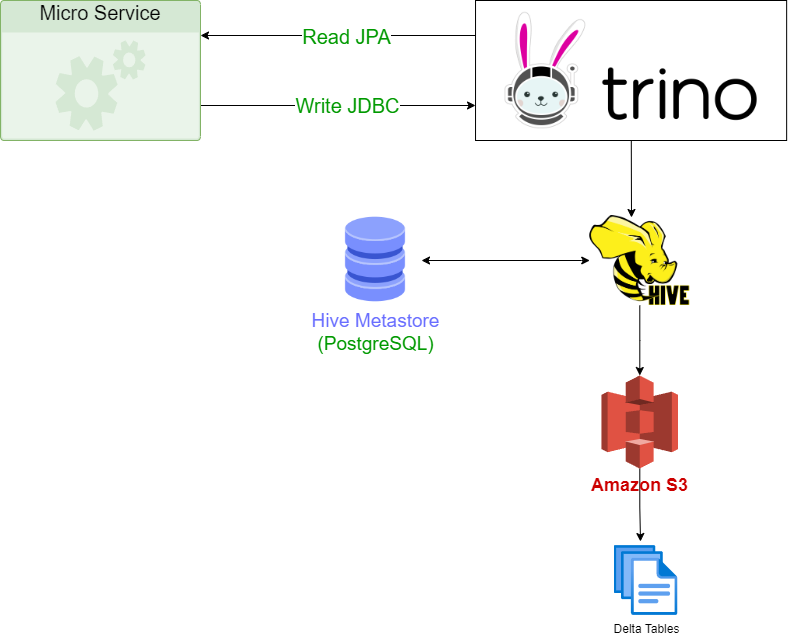
\includegraphics[width=\linewidth]{images/trino_microservice.png}
\caption{TRINO Architecture}\label{fig:arch-trino}
\end{figure}

\begin{figure}[H]
\centering
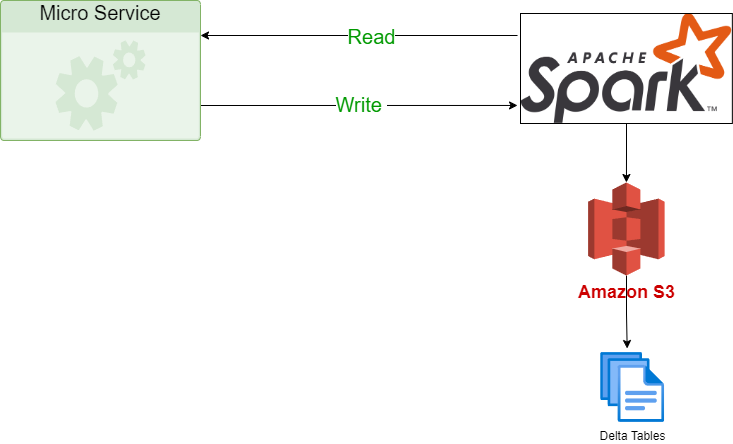
\includegraphics[width=\linewidth]{images/archi-spark.png}
\caption{SPARK Architecture}\label{fig:arch-spark}
\end{figure}

\subsection{Execution Time}
\begin{enumerate}
\item[$\bullet$] \textbf{Trino:} Trino is known for its high execution speed. It uses an optimized architecture to perform SQL queries very quickly by leveraging query parallelization and optimization. Trino can provide short execution times for queries on Delta Lake.
\item[$\bullet$] \textbf{Spark:} Spark is also designed to deliver high performance, but it may require more time to read data from disk. However, Spark can offer high performance when used with complex transformation operations, thanks to its disk-based distributed computing model.
\end{enumerate}

We performed a performance test on a 2-gigabyte Delta table using 2 computers:
\begin{enumerate}
\item The first PC, `DELL Latitude 5530' is where we will launch the following Docker images:
\begin{enumerate}
\item[$\bullet$] \textbf{Trino:} This is the Trino server image for distributed data querying using SQL.
\item[$\bullet$] \textbf{Hive:} It will be used in conjunction with Trino to query and analyze data stored in Hive, thanks to the compatibility between the two systems and the metadata sharing via the Hive Metastore.
\item[$\bullet$] \textbf{PostgreSQL:} It will be used to store metadata of Delta tables, schemas, and partitions, facilitating management, discovery, and access to data in a distributed environment. It also offers query optimization features and permission management to improve data analysis performance and security.
\item[$\bullet$] \textbf{AWS:} Where the Delta tables are located.
\end{enumerate}
\item The second PC, `ASUS ROG G752 VT' is where the Spring Boot microservices for SPARK and TRINO will be executed.
\end{enumerate}

The configuration used in the tests is as follows:
\begin{table}[h]
\centering
\label{tab:caracteristiques}
\begin{tabular}{|l|l|}
\hline
\textbf{Component} & \textbf{Specifications} \\ \hline
Processor & 12th Gen Intel\textsuperscript{®} Core\textsuperscript{TM} i7-1255U 1.70 - 4.8 GHz \\ \hline
Processor Frequency & 2.6 - 3.2 GHz \\ \hline
Memory & 24 GB \\ \hline
Memory Type & DDR4 \\ \hline
Graphics Chip & Intel Iris Xe Graphics \\ \hline
Hard Drive & 512GB PCIe NVMe Class 35 SSD \\ \hline
Operating System Type & Windows 11 64-bit \\ \hline
\end{tabular}
\caption{Technical Specifications of "DELL Latitude 5530" PC}
\end{table}

\begin{table}[h]
\centering
\label{tab:caracteristiques-2}
\begin{tabular}{|l|l|}
\hline
\textbf{Component} & \textbf{Specifications} \\ \hline
Processor & Intel Core i7-6700HQ \\ \hline
Processor Frequency & 2.6 - 3.2 GHz \\ \hline
Memory & 24 GB DDR4 \\ \hline
Hard Drive & 1TB SSD + 1TB HDD \\ \hline
Memory Type & DDR4-SDRAM \\ \\hline
Graphics Chip & Nvidia GeForce GTX 970M \\ \hline
Graphics Memory Quantity & 3072 MB dedicated \\ \hline
Operating System Type & Windows 10 64-bit \\ \hline
\end{tabular}
\caption{Technical Specifications of `ASUS ROG G752 VT' PC}
\end{table}

The results are as follows:

\begin{table}[h]
\centering
\label{tab:resultats}
\begin{tabular}{|l|l|l|}
\hline
\multirow{2}{*}{\textbf{Queries}} & \multicolumn{2}{c|}{\textbf{Implementation}} \\ \cline{2-3}
& \textbf{Spark (s)} & \textbf{Trino (s)} \\ \hline
SELECT (per page and per page result limit - 100 per page) & 1.2 & 0.43 \\ \hline
Aggregation and grouping & 2.1 & 0.8 \\ \hline
Sorting & 2.2 & 0.8 \\ \hline
\end{tabular}
\caption{Technical Specifications of `ASUS ROG G752 VT' PC}
\end{table}

\subsection{Memory Management}
\begin{enumerate}
\item[$\bullet$] \textbf{Trino:} Trino primarily utilizes memory to accelerate query processing. It has an in-memory query engine that optimizes data access and minimizes access times. However, this means that Trino may require a significant amount of memory to process large datasets.
\item[$\bullet$] \textbf{Spark:} Spark uses a disk-based distributed computing model, which means data is typically stored on disk and loaded into memory as needed. This allows Spark to handle much larger datasets than what can fit in memory.
\end{enumerate}

\subsection{Ecosystem and Integrations}
\begin{enumerate}
\item[$\bullet$] \textbf{Trino:} Trino has a growing ecosystem with a wide range of connectors and integrations, allowing access to different data sources, including Delta Lake. It is compatible with various data visualization and processing tools.
\item[$\bullet$] \textbf{Spark:} Spark is a mature project with a rich ecosystem of tools, libraries, and connectors. It benefits from a large developer community and numerous learning resources. Spark also supports both stream processing and batch processing of data.
\end{enumerate}

\subsection{Scalability}
\begin{enumerate}
\item[$\bullet$] \textbf{Trino:} Trino is designed to be highly scalable and can handle large datasets. It can be easily configured to accommodate intensive workloads and significant data volumes.
\item[$\bullet$] \textbf{Spark:} Spark is also designed for scalability and can process massive datasets. It has a distributed processing system that can adapt to different cluster configurations and resources.
\end{enumerate}

\subsection{Support for Delta Lake Features}
\begin{enumerate}
\item[$\bullet$] \textbf{Trino:} Trino has an official connector for Delta Lake, allowing it to read and write data in Delta Lake. It supports essential Delta Lake features such as ACID transaction management, incremental updates, and merge operations.
\item[$\bullet$] \textbf{Spark:} Spark also has built-in support for Delta Lake. It offers advanced Delta data management features, including support for ACID transactions, efficient merge operations, and data versioning mechanisms.
\end{enumerate}

\subsection{Ease of Use}
\begin{enumerate}
\item[$\bullet$] \textbf{Trino:} Trino provides a standard SQL interface, making it easy to use for users familiar with SQL. It also offers user-friendly interactive querying tools and flexible configuration options.
\item[$\bullet$] \textbf{Spark:} Spark offers an SQL interface through Spark SQL, but it is also oriented towards data processing through a broader API. Spark may be more complex to use for users less familiar with distributed processing concepts.
\end{enumerate}

\subsection{Other Statistics}

\begin{longtable}{|p{0.23\linewidth}|p{0.35\linewidth}|p{0.42\linewidth}|}
\hline
\textbf{} & \textbf{Spark} & \textbf{Trino} \\ \hline
\textbf{Developer Experience} & 

\includegraphics[width=0.28in,height=0.28in]{images/image3.png}
\includegraphics[width=0.28in,height=0.28in]{images/image3.png}\newline
Spark's syntax requires SMEs to have experience in data engineering &

\includegraphics[width=0.28in,height=0.28in]{images/image3.png}
\includegraphics[width=0.28in,height=0.28in]{images/image3.png}
\includegraphics[width=0.28in,height=0.28in]{images/image3.png}\newline
Standard SQL interface, making it easier to use for users familiar with SQL. \\ \hline
\textbf{Coût} & 
Team: 
\includegraphics[width=0.33in,height=0.35in]{images/image4.jpg}
\includegraphics[width=0.33in,height=0.35in]{images/image4.jpg}\newline
Infrastructure: \textcolor[RGB]{0, 128, 0}{\textbf{\large \$}} & 
Team: 
\includegraphics[width=0.33in,height=0.35in]{images/image4.jpg}
\includegraphics[width=0.33in,height=0.35in]{images/image4.jpg}\newline
Infrastructure: \textcolor[RGB]{0, 128, 0}{\textbf{\large \$}} \\ \hline
\textbf{Fiabilité} & 

\includegraphics[width=0.28in,height=0.28in]{images/image3.png}
\includegraphics[width=0.28in,height=0.28in]{images/image3.png}
\includegraphics[width=0.28in,height=0.28in]{images/image3.png}\newline
Mature product maintained internally and supported by Google Dataproc &

\includegraphics[width=0.28in,height=0.28in]{images/image3.png}
\includegraphics[width=0.28in,height=0.28in]{images/image3.png}\newline
Has experienced a few outages as the internal team learns to maintain and scale \\ \hline
\textbf{Caractéristiques et Open sources} & 

\includegraphics[width=0.28in,height=0.28in]{images/image3.png}
\includegraphics[width=0.28in,height=0.28in]{images/image3.png}
\includegraphics[width=0.28in,height=0.28in]{images/image3.png}\newline
Has been supported by the open-source community since 2014. &

\includegraphics[width=0.28in,height=0.28in]{images/image3.png}
\includegraphics[width=0.28in,height=0.28in]{images/image3.png}
\includegraphics[width=0.28in,height=0.28in]{images/image3.png}\newline
Has been supported by the open-source community since 2019. Shopify has made contributions \\ \hline
\textbf{Usage} & 
\textasciitilde Approximately 800,000 jobs/day &
3000 active users/week \newline
\textasciitilde Approximately 200,000 queries/week \\ \hline
\end{longtable}

\section{Solution Design}

For the solution design, we have chosen an architecture based on microservices, using the following technologies: Spring Data, JPA, Hibernate, JDBC, and Trino.

The microservices are developed using Spring Data, which provides a high-level abstraction for interacting with the database. This allows the use of annotations and interfaces to define entities, queries, and persistence operations. JPA (Java Persistence API) is used as the interface layer for interacting with the database, while Hibernate is used as the persistence provider, enabling the management of Java objects and their mapping to Trino.

Communication between the microservices is facilitated by a Kafka broker. Kafka is a distributed streaming platform that allows microservices to exchange messages in real-time. Microservices publish events to Kafka topics, and other microservices can subscribe to these topics to receive the corresponding events.

For authentication and authorization management, we use Spring Cloud Gateway. This component receives service calls from web, mobile, or desktop applications. These applications send a JSON Web Token (JWT) to Spring Cloud Gateway for authentication. Spring Cloud Gateway verifies the availability of the token by contacting Keycloak, which is responsible for identity and access management. Once the token is validated, Spring Cloud Gateway allows the request to pass through to the microservices.

The microservices communicate with Trino using the JDBC connector. Trino is responsible for querying and processing data from a large number of data sources. It stores metadata in Hive, which is a data warehouse based on Hadoop. Trino also uses the concept of Delta tables to manage incremental data changes. These Delta tables are stored on AWS (Amazon Web Services), providing a scalable and reliable storage solution.

\begin{figure}[H]
\centering
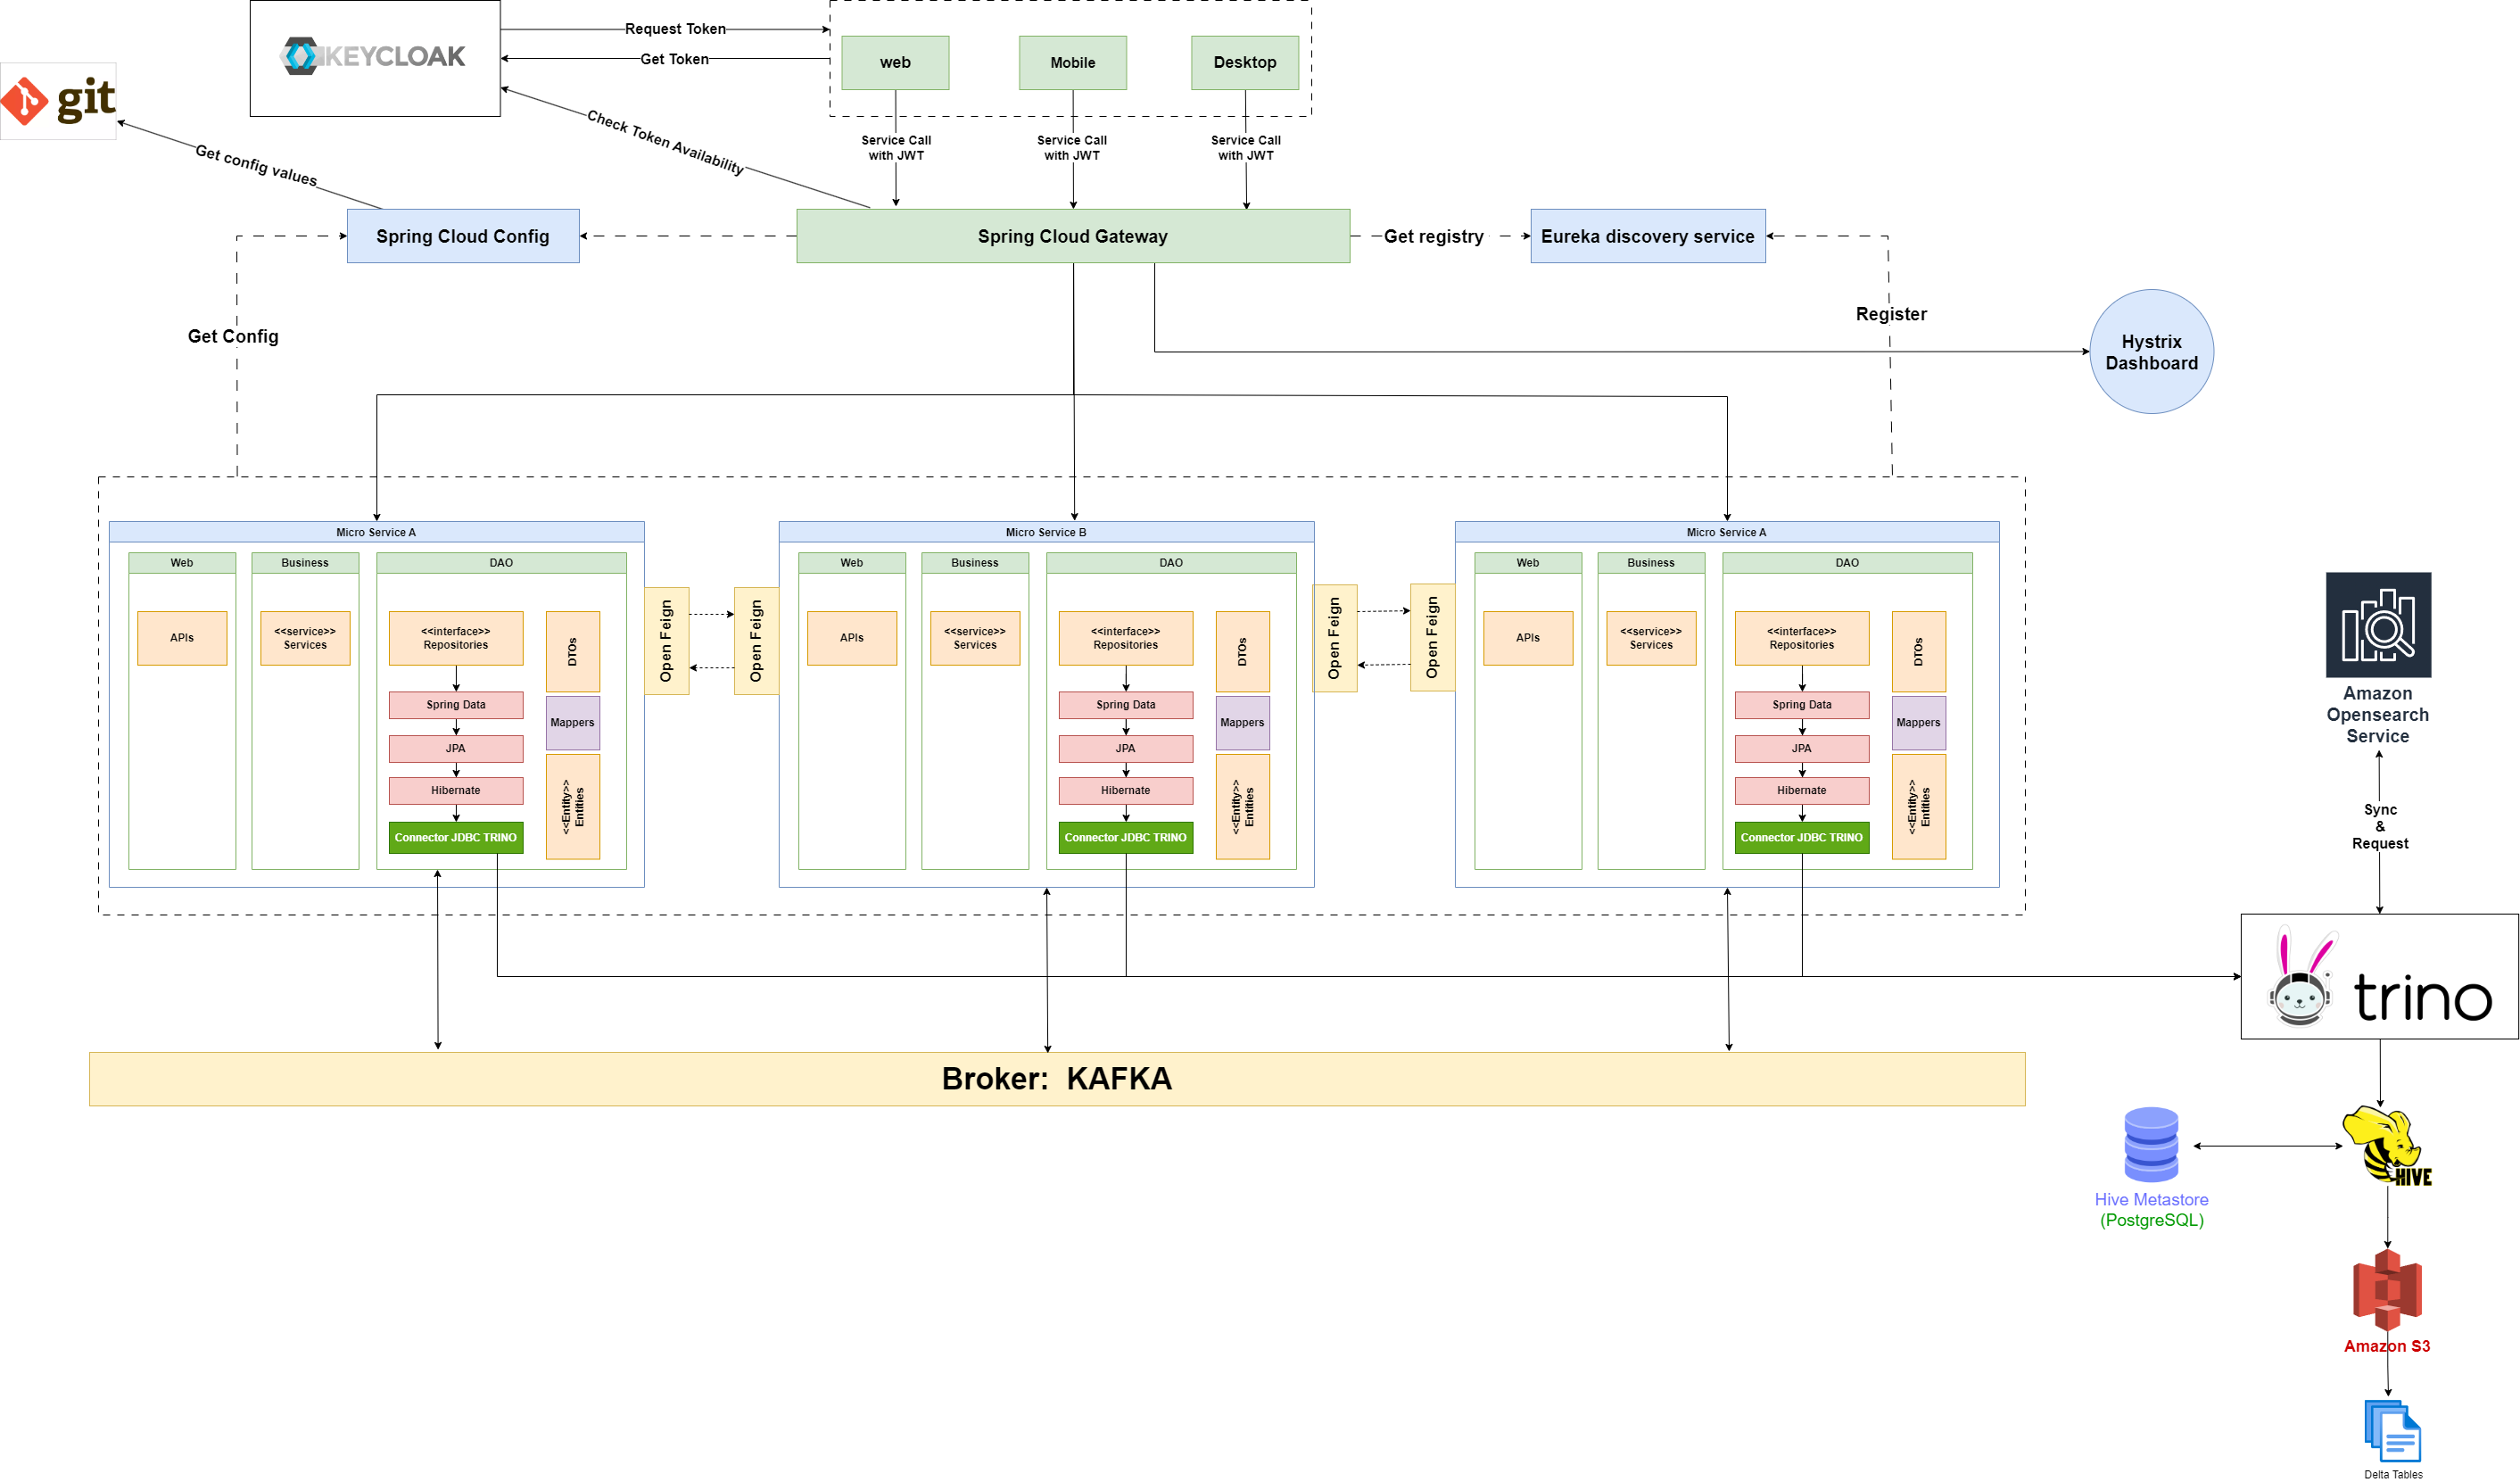
\includegraphics[width=\linewidth]{images/architecture-solution.png}
\caption{Solution Architecture}\label{fig:solution}
\end{figure}

\section{Advantages}

The chosen architecture offers several significant advantages:

\begin{enumerate}
\item[$\bullet$] \textbf{Scalability:} The microservices-based architecture allows for horizontal scalability, meaning each microservice can be deployed and scaled independently based on its specific needs. This enables fine-grained capacity and resource adjustments, making it easier to handle high workloads and adapt to growing application requirements.
\item[$\bullet$] \textbf{Modularity:} The modular design of microservices enables more efficient development, deployment, and maintenance. Each microservice can be developed independently, facilitating collaboration between teams and promoting code reuse. Additionally, modifications or updates to one microservice do not impact others, reducing the risks of errors and conflicts.
\item[$\bullet$] \textbf{Technological Flexibility:} Microservices provide flexibility in terms of technological choices. Each microservice can be developed using the most suitable technologies for its specific functionality. This allows for leveraging the advantages of each technology and selecting the best tools for each component of the architecture.
\item[$\bullet$] \textbf{Effective Communication:} Using Kafka as a streaming broker facilitates communication between microservices. Kafka ensures reliability and scalability of real-time event exchanges, enabling smooth communication and efficient synchronization between different system components.
\item[$\bullet$] \textbf{Enhanced Security:} Integration of Keycloak for authentication and authorization provides a high level of security. JWT tokens are used for user identification, and Spring Cloud Gateway handles token verification and management. This ensures that only authorized individuals have access to appropriate resources and functionalities, strengthening application security.
\item[$\bullet$] \textbf{Optimized Performance:} Utilizing Trino as a distributed query engine allows querying and processing large amounts of data in a parallel and efficient manner. Trino offers high performance and query optimization, enabling faster results and improved user experience.
\end{enumerate}

These advantages contribute to a scalable, modular, flexible, secure, and high-performing architecture that meets the requirements of your project.

\section{Visualization}

In this section, we will present screenshots of the different microservices in our solution, including Swagger for the API, the Trino console for data exploration, and the Izicap website. These screenshots will illustrate the user interface and the functionalities offered by each service.

\subsection{Trino Console}

\begin{figure}[H]
\centering
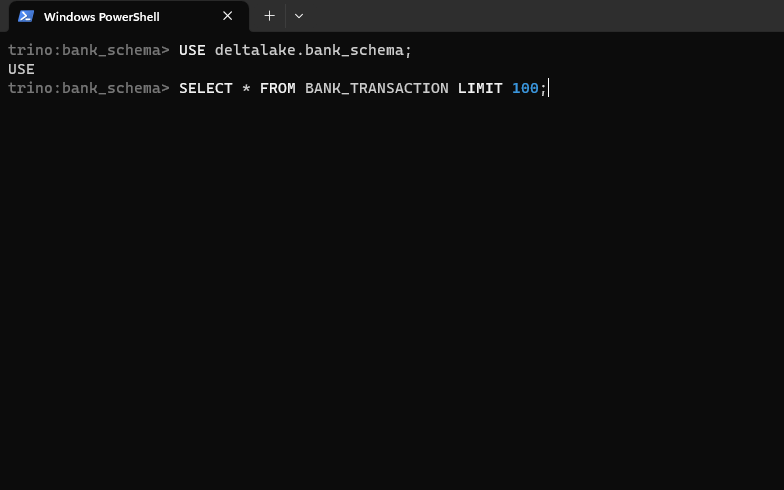
\includegraphics[width=\linewidth]{images/trino-1.png}
\caption{Trino Console}\label{fig:trino-1}
\end{figure}

\begin{figure}[H]
\centering
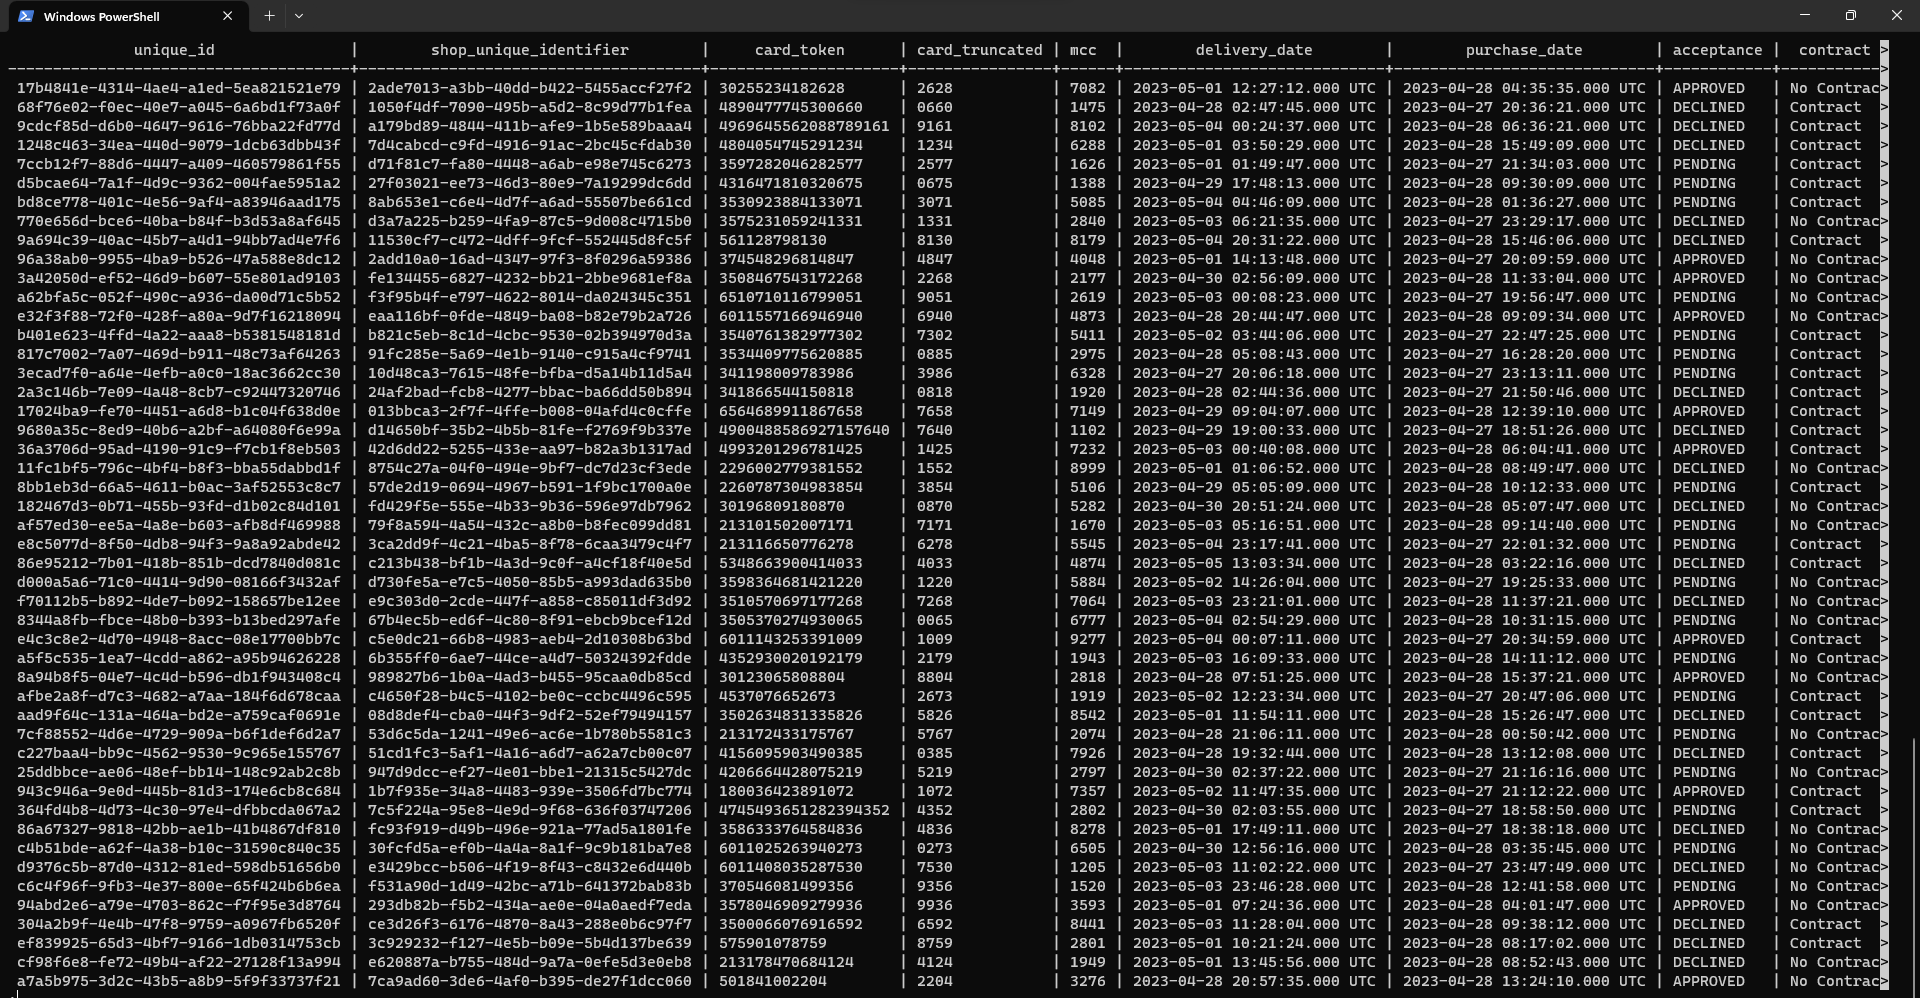
\includegraphics[width=\linewidth]{images/trino-2.png}
\caption{Trino SELECT Query}\label{fig:trino-2}
\end{figure}

\begin{figure}[H]
\centering
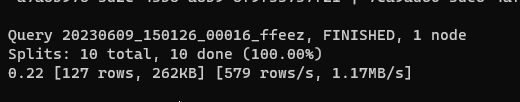
\includegraphics[width=\linewidth]{images/trino-3.png}
\caption{Trino command prompt}\label{fig:trino-3}
\end{figure}

These screenshots of the Trino console highlight the advanced data querying interface provided by Trino. Developers and analysts can execute SQL queries on the data stored in Trino, explore schemas, preview results, and perform analytical operations to extract valuable insights.

\subsection{Microservices}

\begin{figure}[H]
\centering
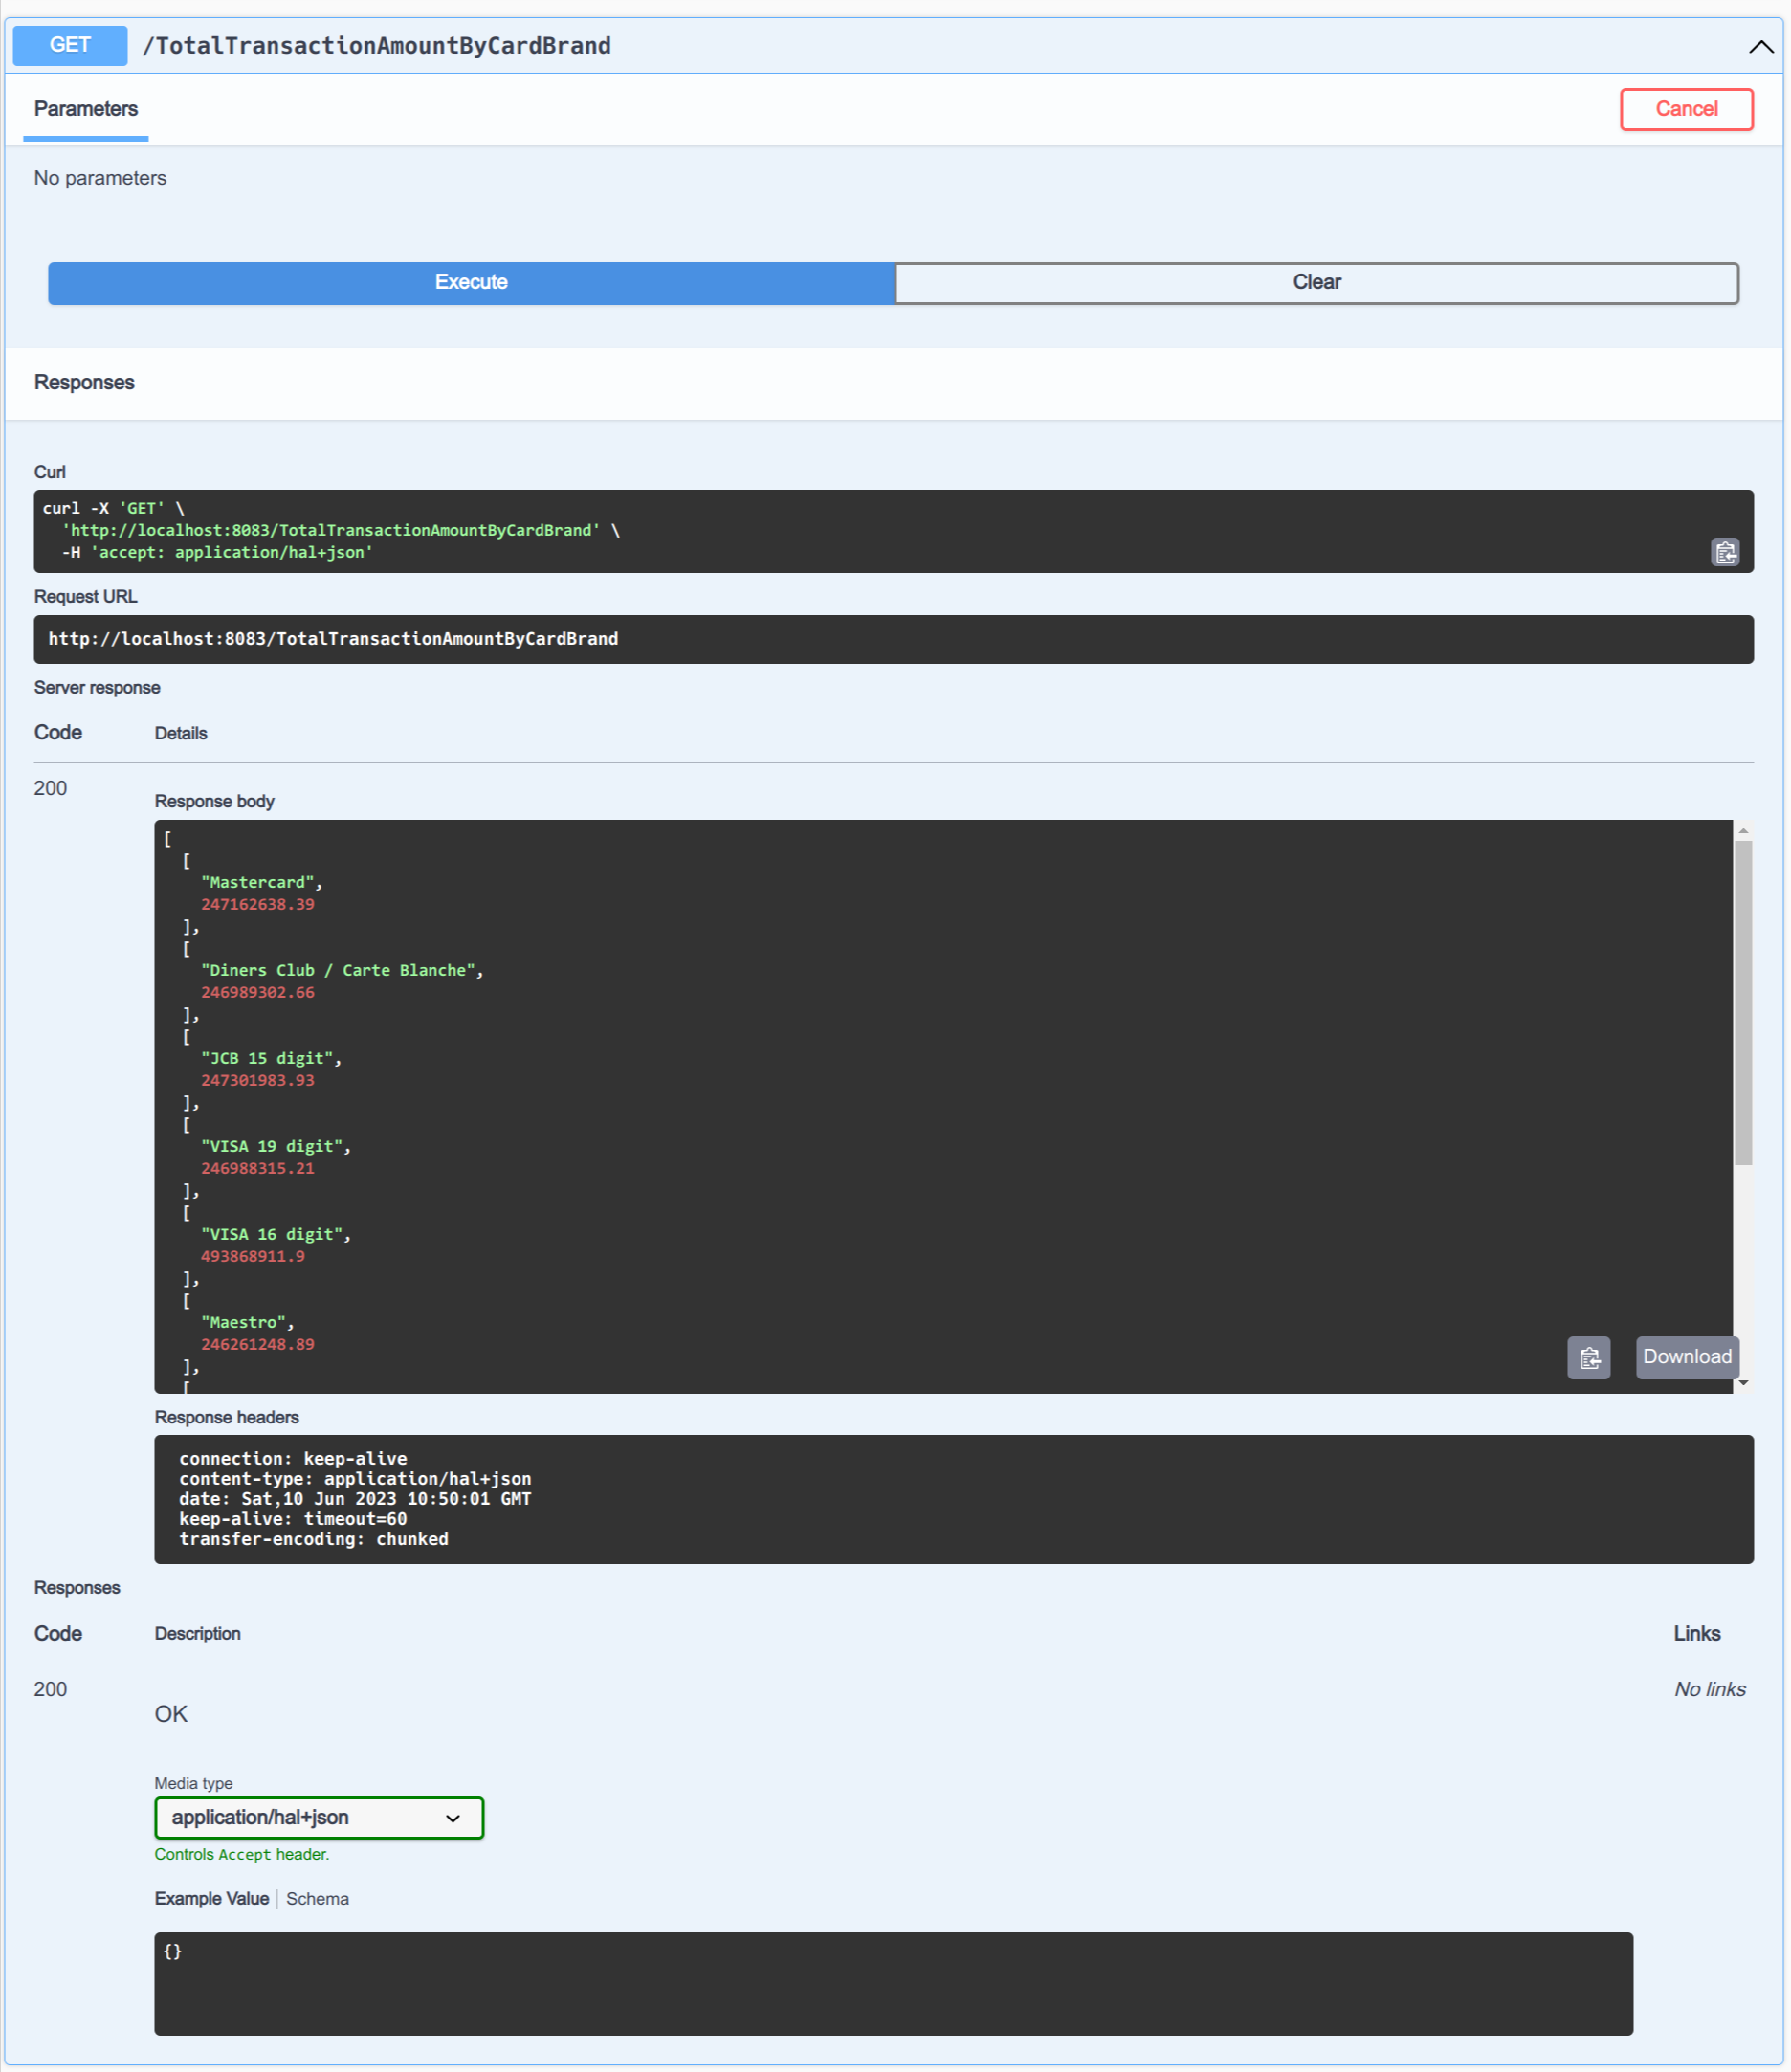
\includegraphics[width=\linewidth]{images/Swagger-UI-1.png}
\caption{Swagger UI of Endpoint 1}\label{fig:swagger-1}
\end{figure}

\begin{figure}[H]
\centering
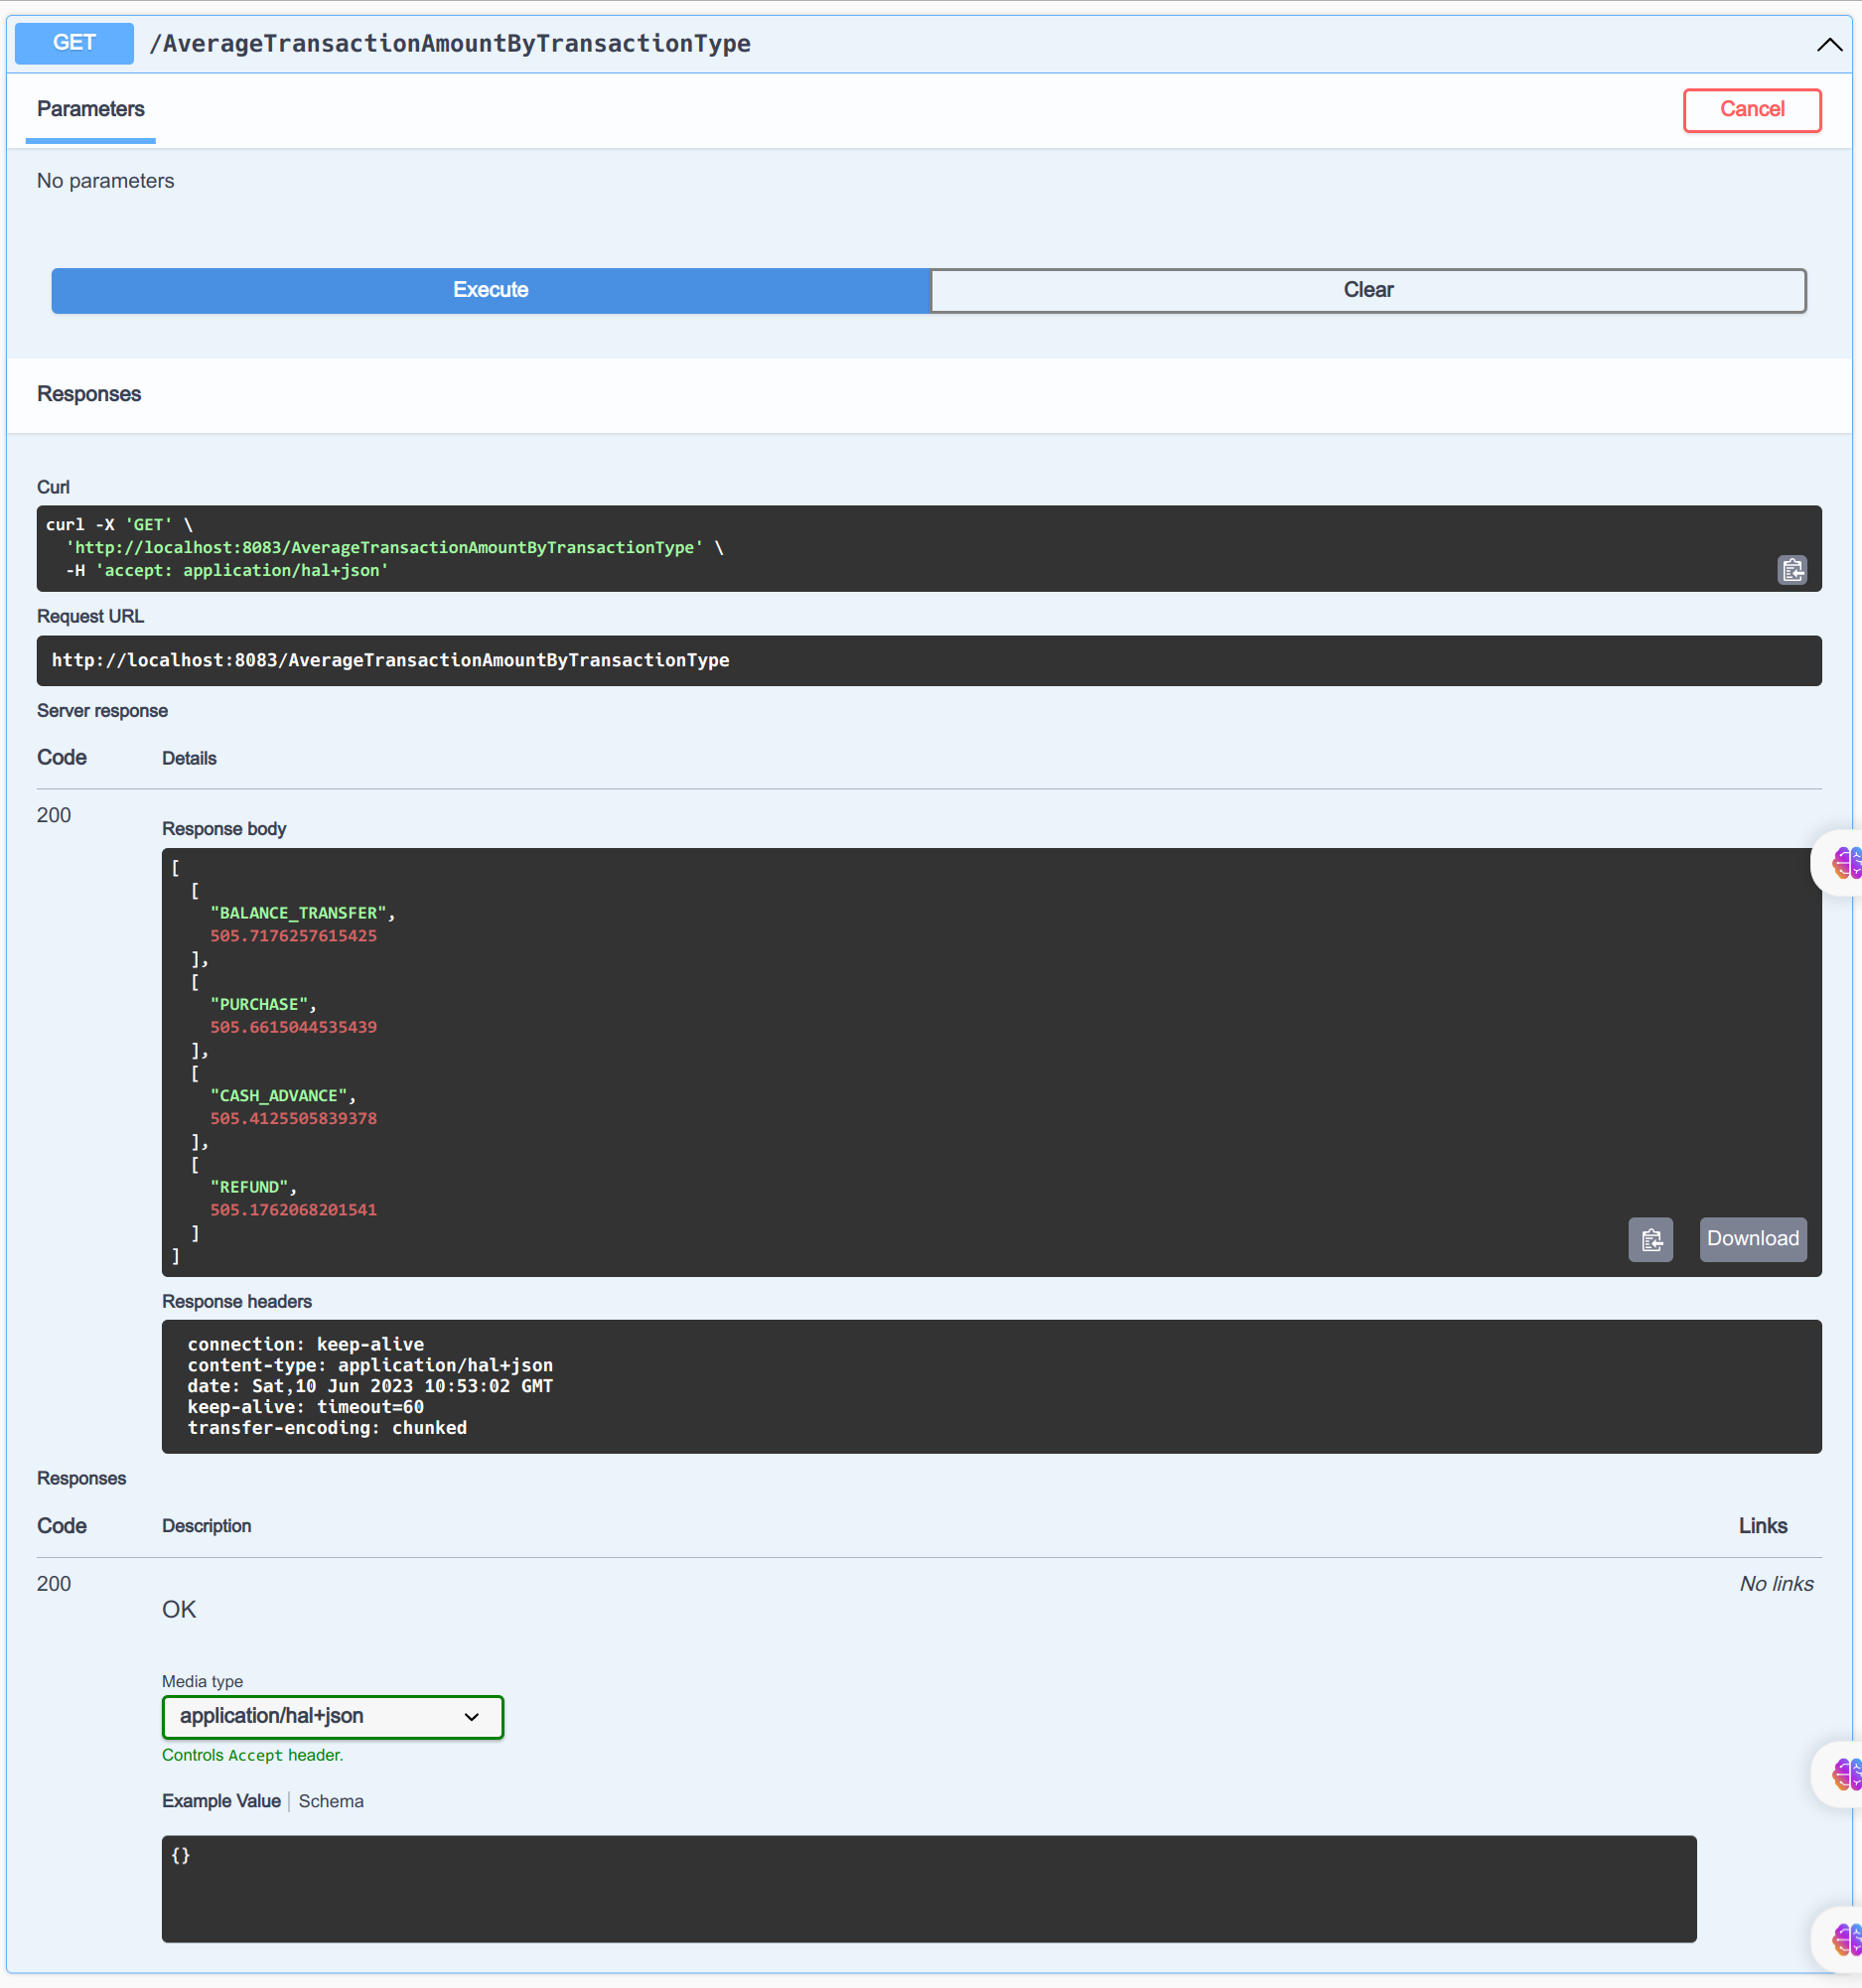
\includegraphics[width=\linewidth]{images/Swagger-UI-2.png}
\caption{Swagger UI of Endpoint 2}\label{fig:swagger-2}
\end{figure}

\begin{figure}[H]
\centering
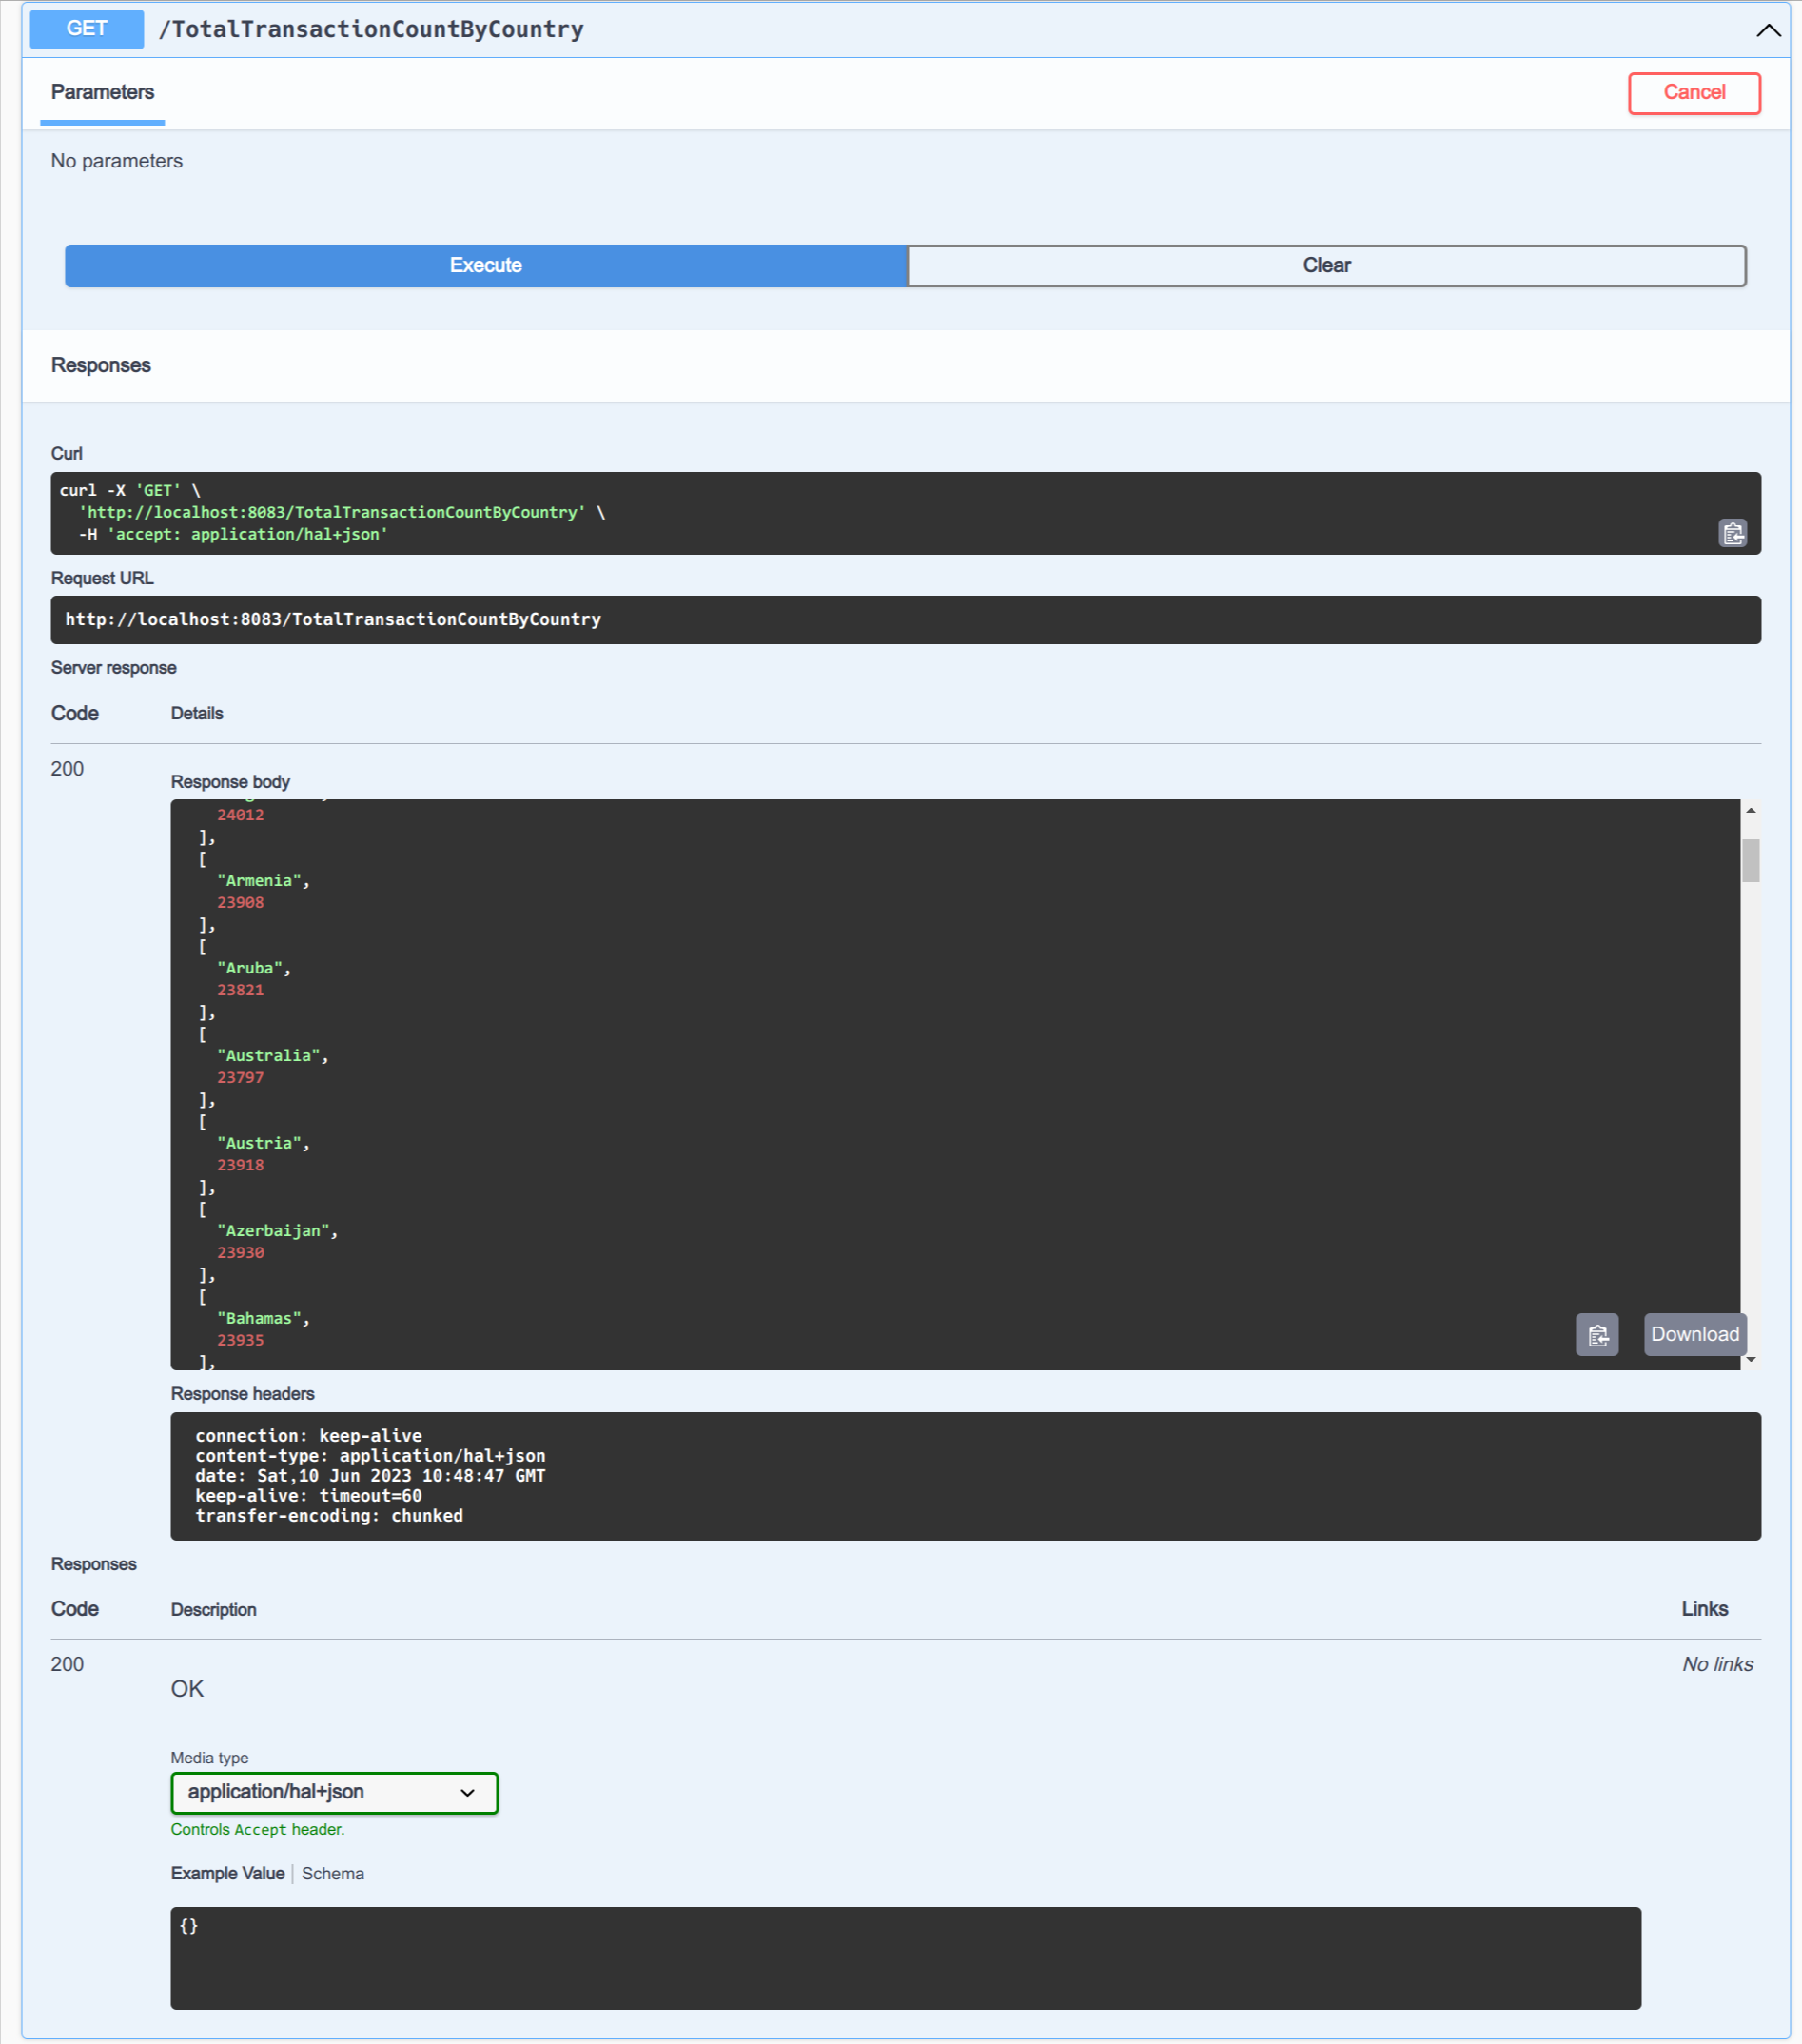
\includegraphics[width=\linewidth]{images/Swagger-UI.png}
\caption{Swagger UI of Endpoint 3}\label{fig:swagger-3}
\end{figure}

\begin{figure}[H]
\centering
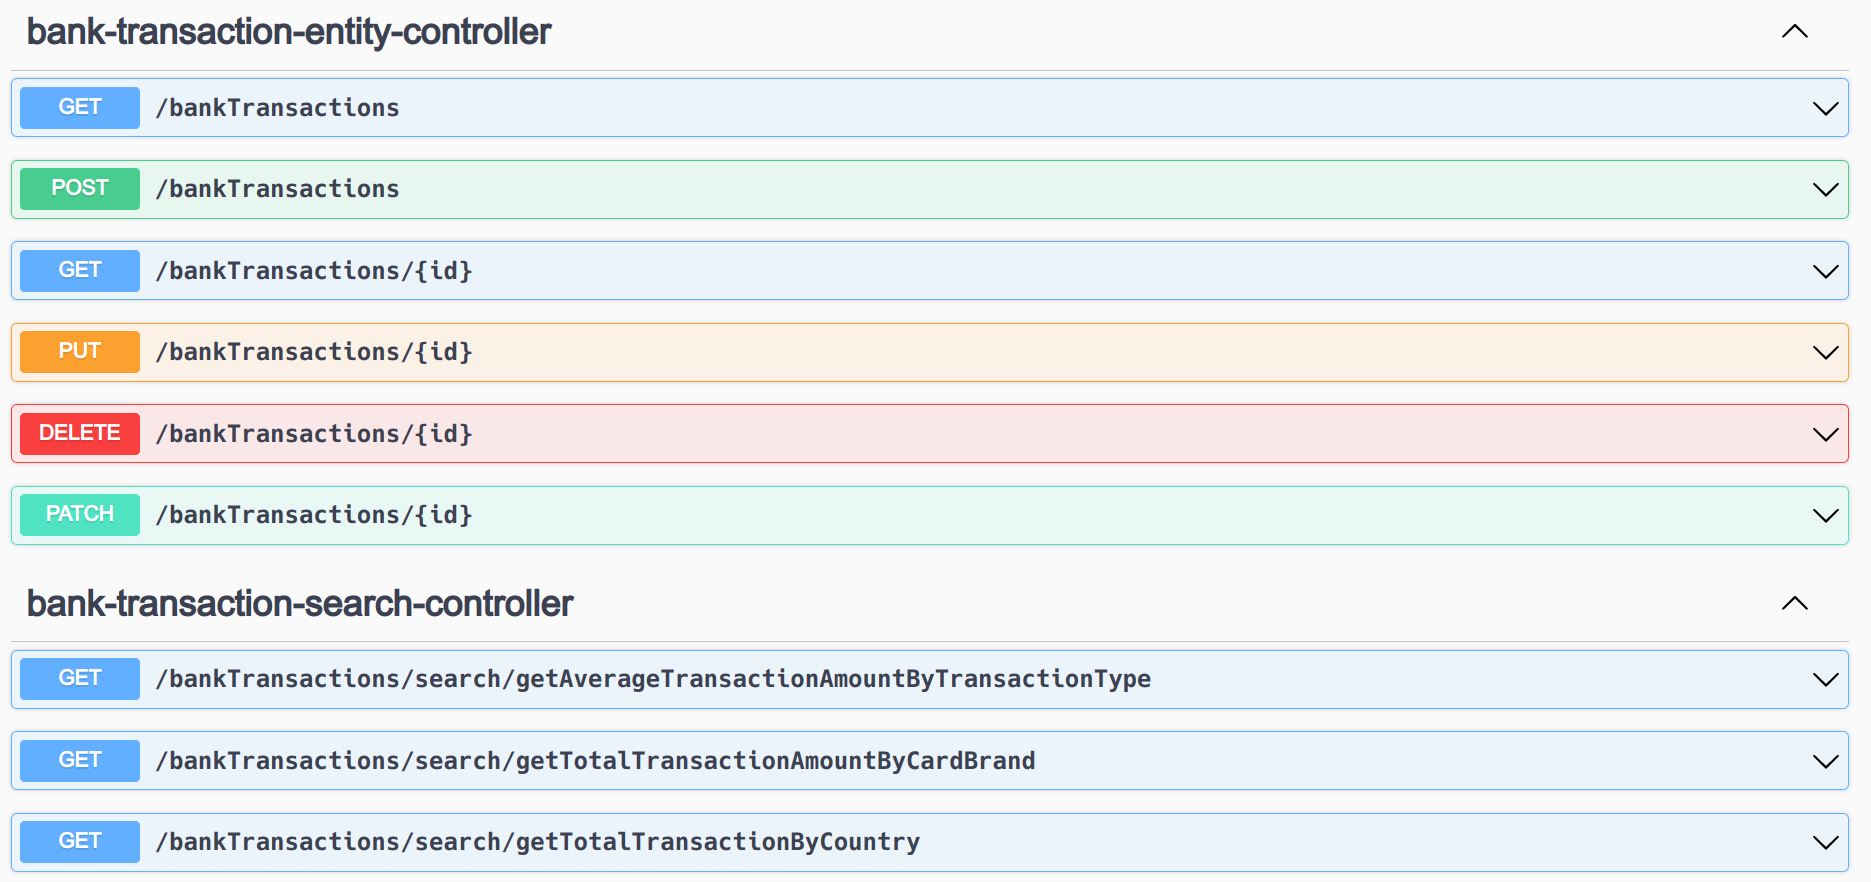
\includegraphics[width=\linewidth]{images/Swagger-UI-3.png}
\caption{Swagger UI}\label{fig:swagger-4}
\end{figure}

These images showcase the detailed documentation of our API using Swagger. This user-friendly interface allows developers to understand the available endpoints, required parameters, expected responses, and usage examples. Swagger facilitates integration and communication with our microservices.

\subsection{Delta Lake}

\begin{figure}[H]
\centering
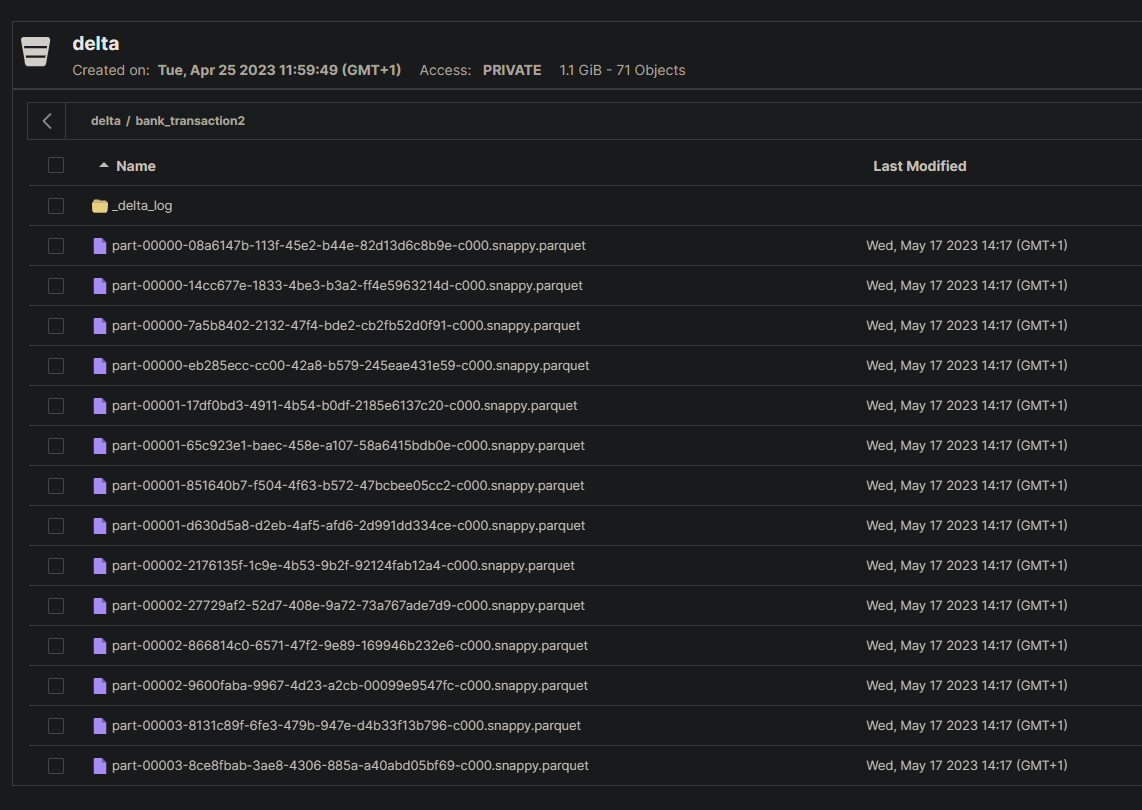
\includegraphics[width=\linewidth]{images/delta-lake-dossier.png}
\caption{Parquet Data}\label{fig:delta-lake-folder}
\end{figure}

We have data files in the Parquet format. Parquet files are optimized for efficient storage and retrieval of data. They are compressed and structured in a way that allows for fast queries and selective reading of data. These Parquet files contain the actual table data, organized into columns and partitions, making it easy to manipulate and further analyze the data.

\subsection{Izicap UI}

\begin{figure}[H]
\centering
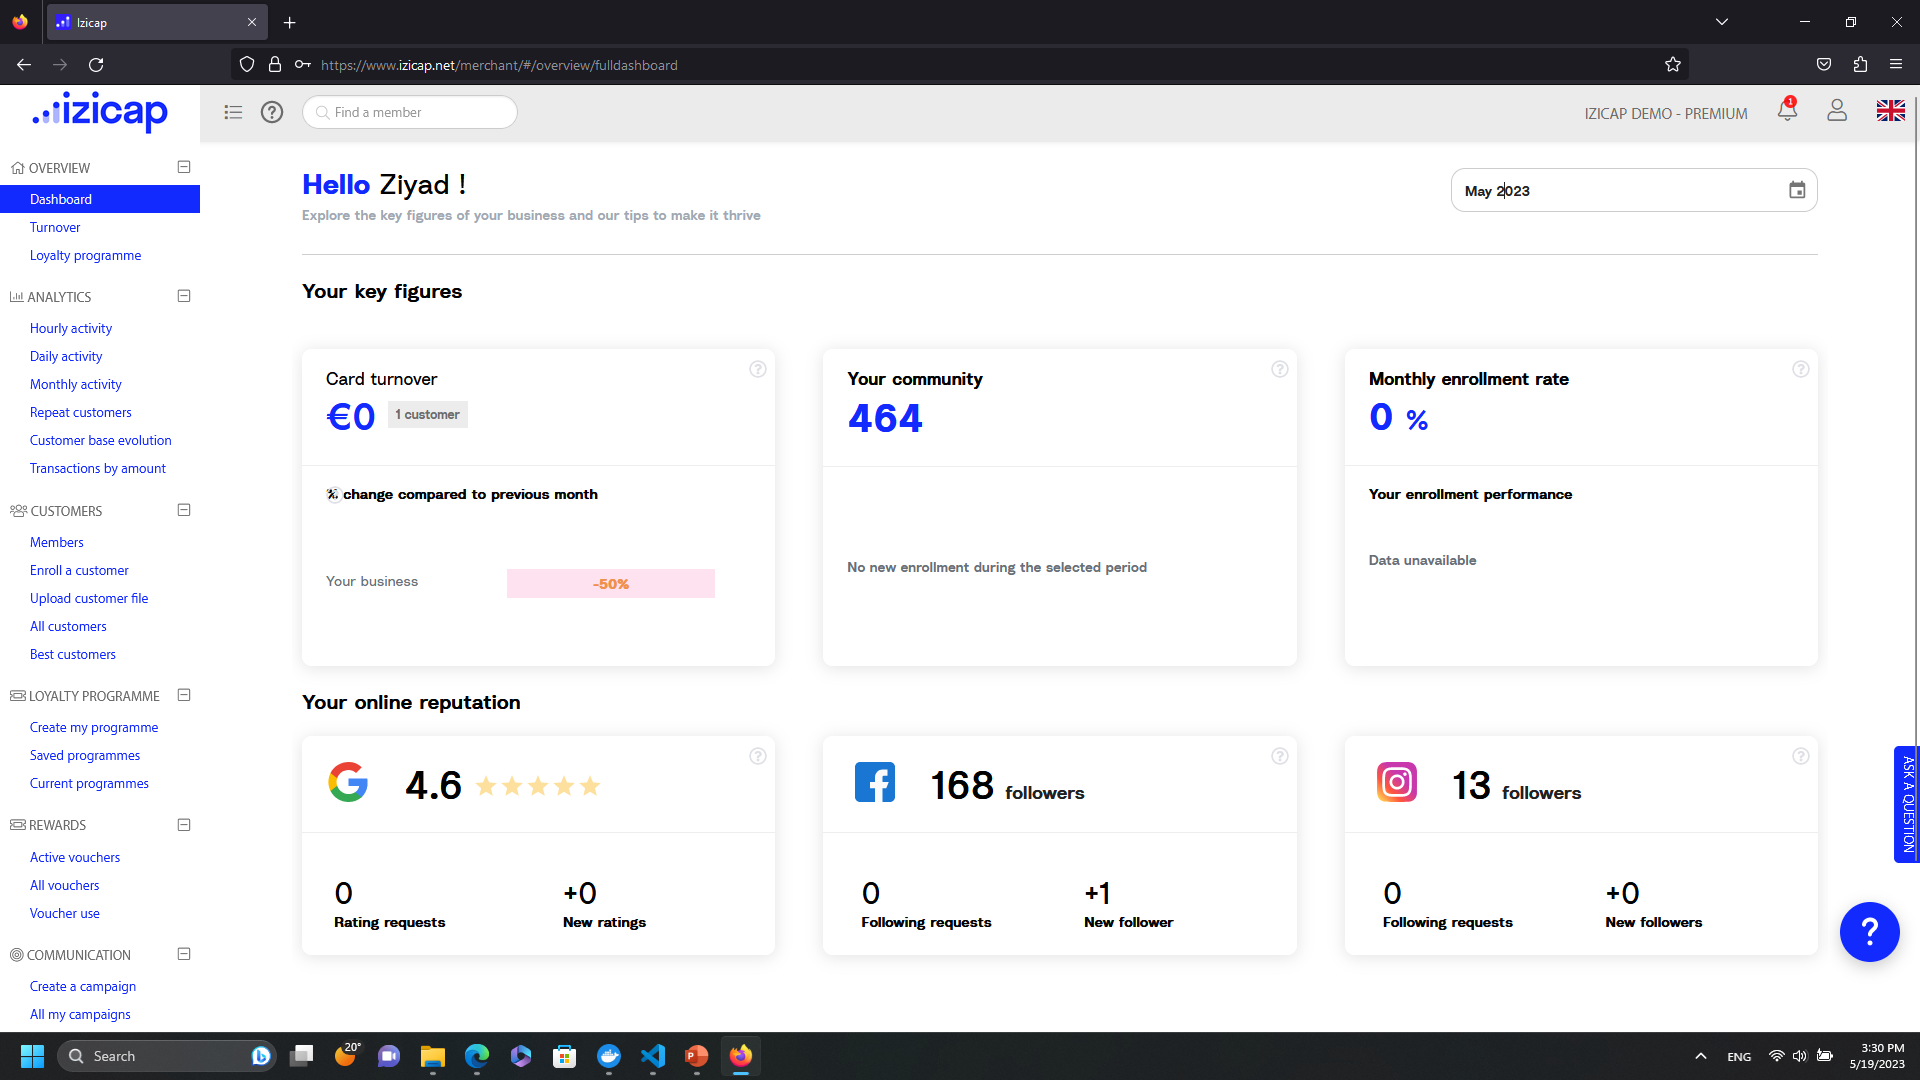
\includegraphics[width=\linewidth]{images/izicap-portail.png}
\caption{Izicap Portal}\label{fig:izicap-1}
\end{figure}

\begin{figure}[H]
\centering
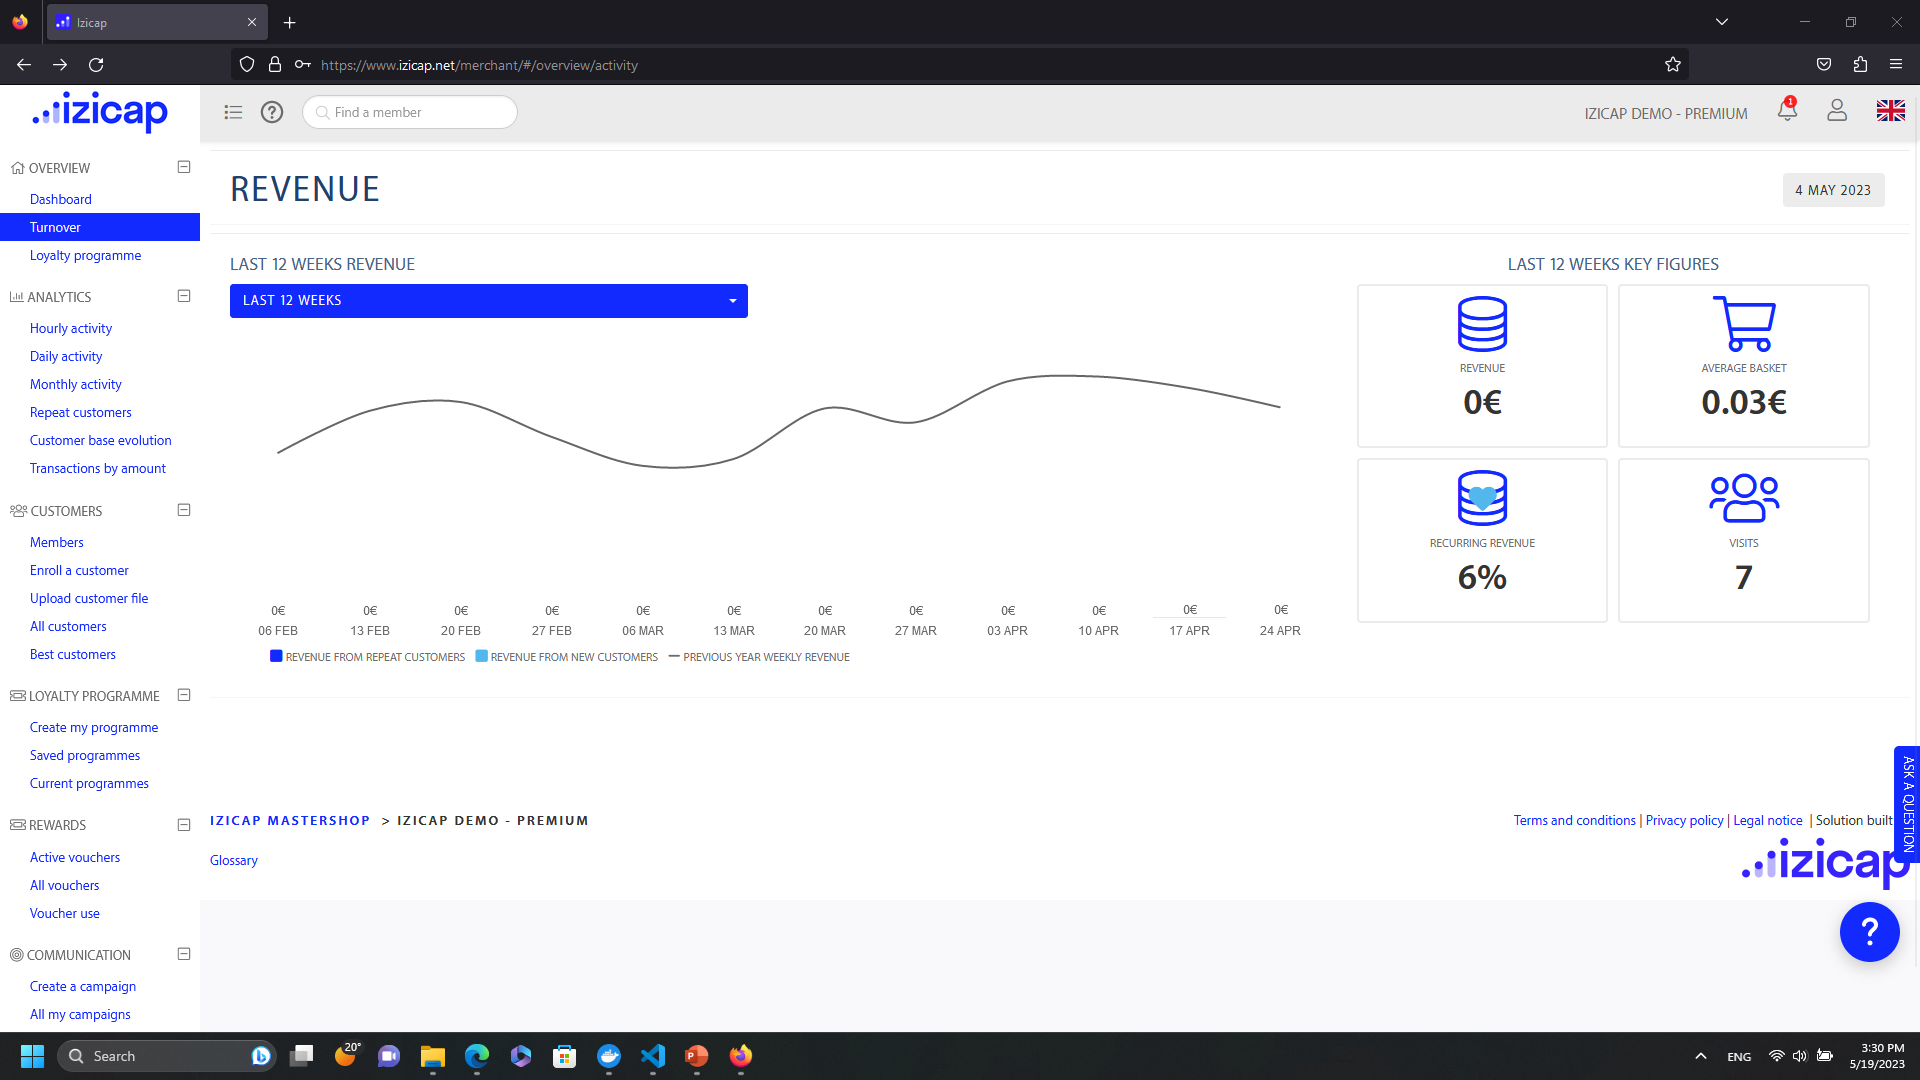
\includegraphics[width=\linewidth]{images/revenu.png}
\caption{Customer Revenue}\label{fig:izicap-2}
\end{figure}

\begin{figure}[H]
\centering
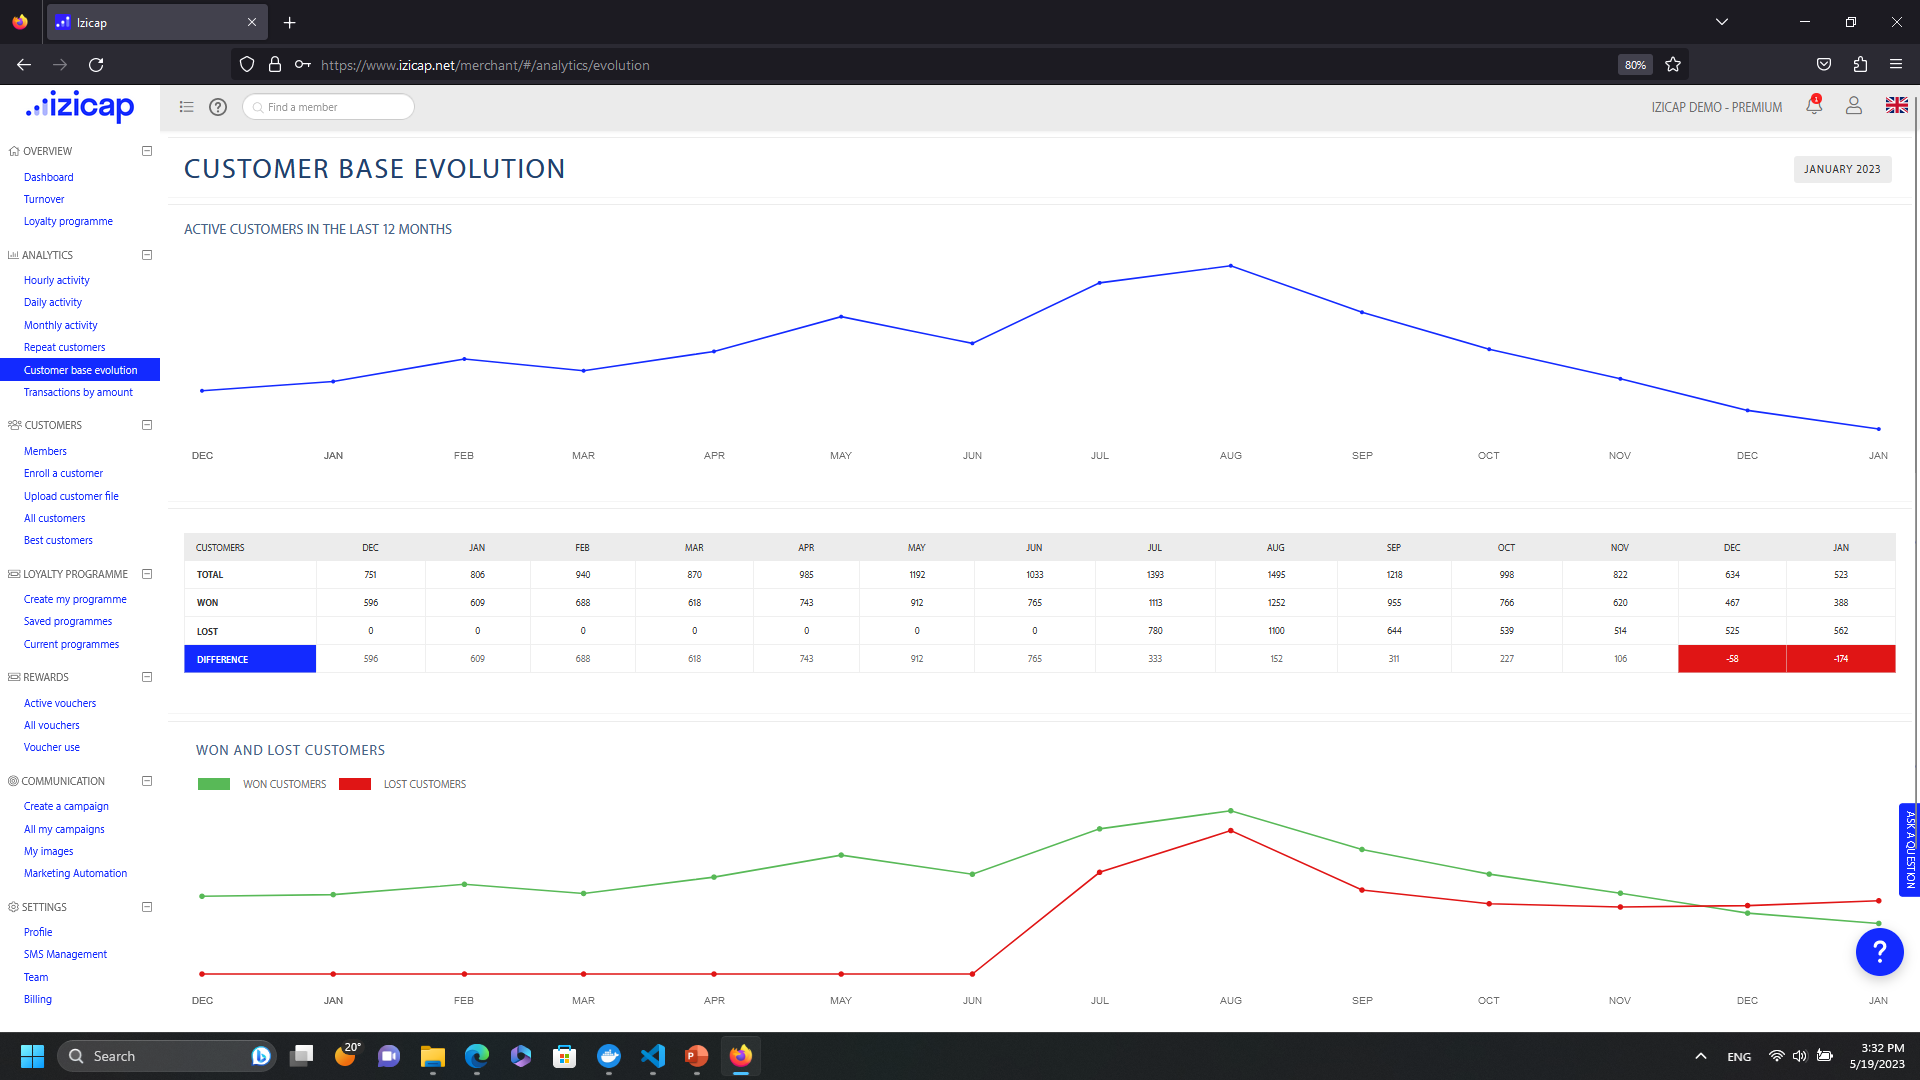
\includegraphics[width=\linewidth]{images/data-1.png}
\caption{Customer Base Evolution}\label{fig:izicap-3}
\end{figure}

\begin{figure}[H]
\centering
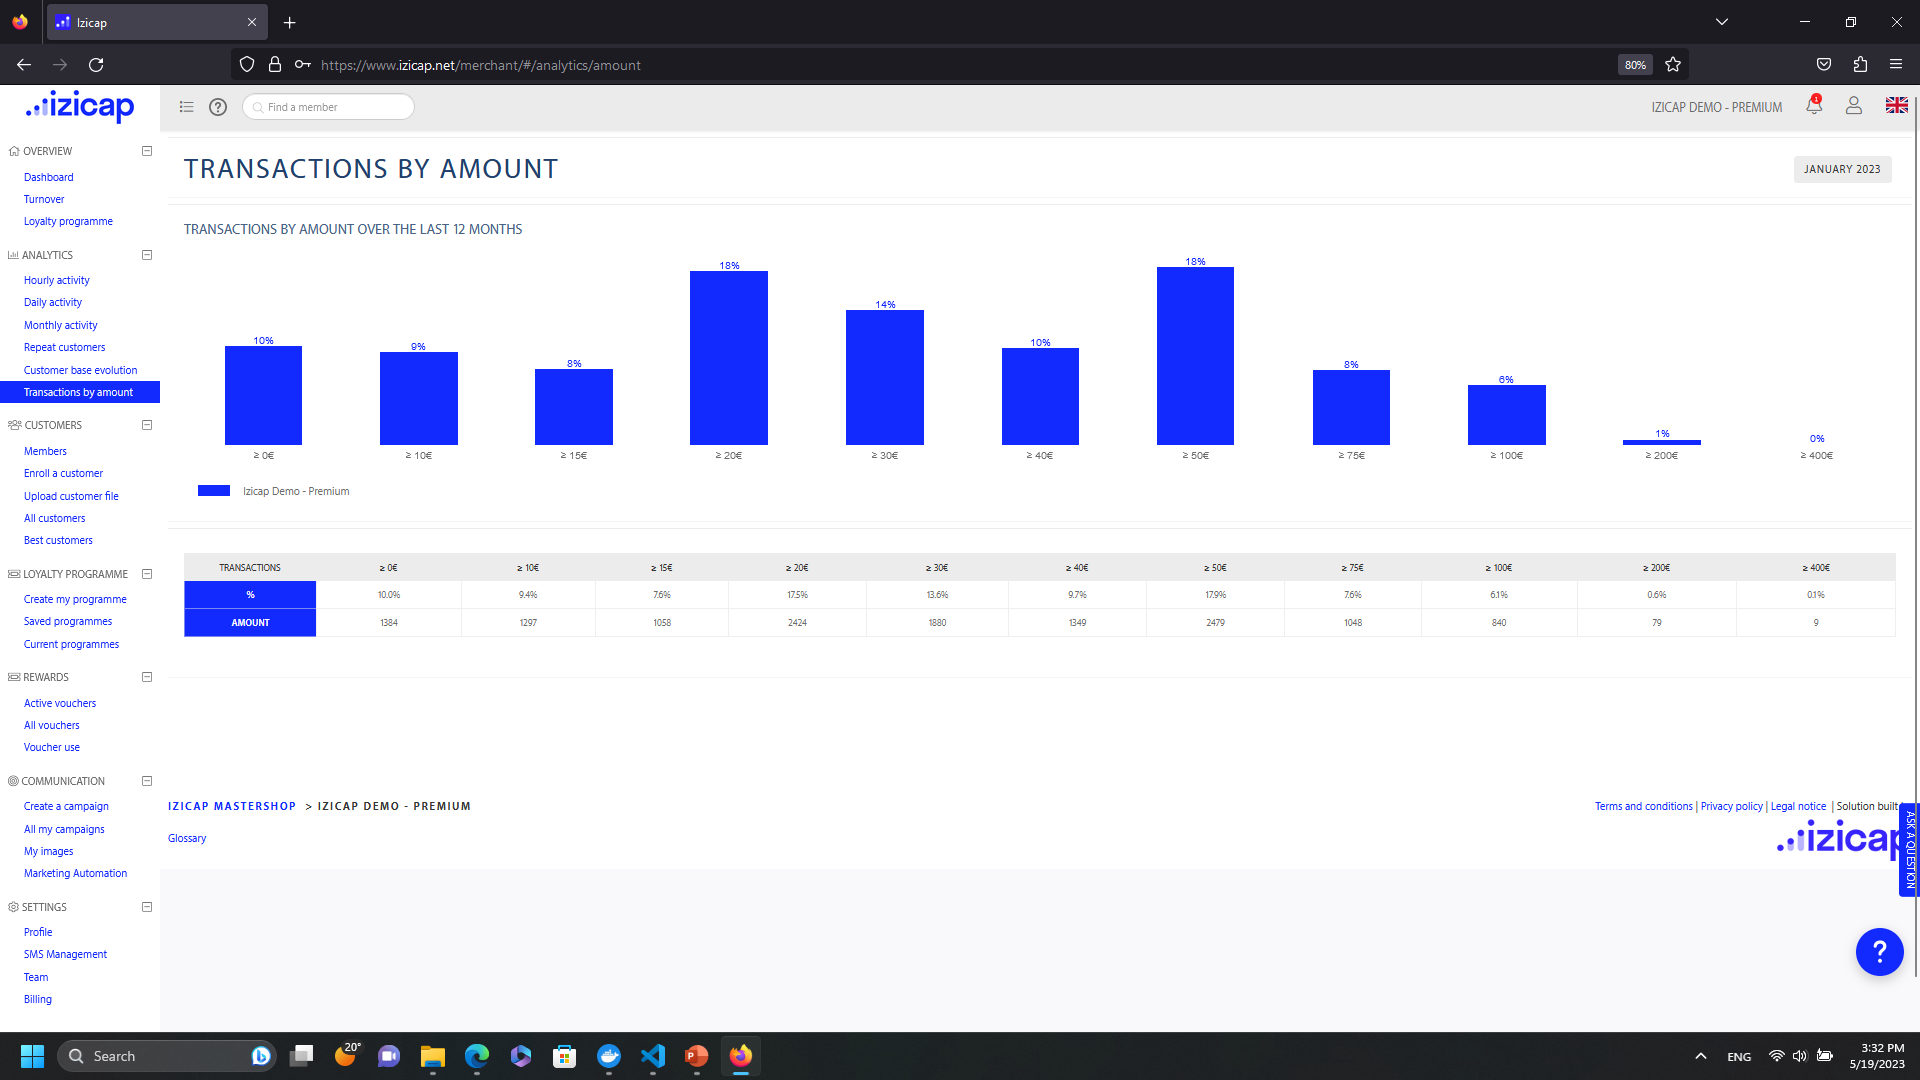
\includegraphics[width=\linewidth]{images/data-2.png}
\caption{Transactions by Amount}\label{fig:izicap-4}
\end{figure}

The use of micro-frontends allows for splitting the user interface into several independent modules, each being responsible for a specific functionality. This enables clear separation of responsibilities and facilitates the development, maintenance, and evolution of the application.

\section*{Conclusion}
The feasibility study of connectors for manipulating Delta Lake has allowed us to make informed decisions regarding the implementation of the solution. While Spark is widely used and integrated into the Big Data ecosystem, Trino offers significant advantages in terms of flexibility and performance for SQL queries. Based on our specific needs and technical constraints, we have chosen to use Trino as the connector for manipulating Delta Lake in our solution.